{\fontsize{12}{14}\selectfont 
\begin{figure}[H]
  \centering
  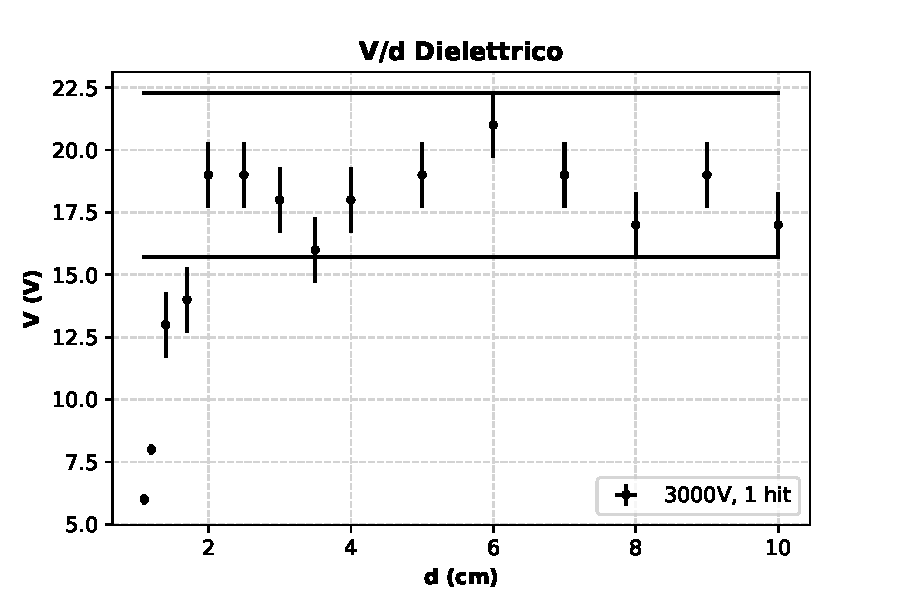
\includegraphics[width=13cm]{Figures/Grafico_Parte4.pdf}
  \caption{Grafico della tensione (in Volt) in funzione della distanza tra le piastre (in cm). L'errore sulla tensione è pari a $1\% $f.s. + $1$ digit, mentre l'errore sulla distanza è di $1 mm$. Sono state tracciate due rette asintotiche nei punti in cui la tensione è arrivata a saturazione. Da queste, facendone la semisomma e la semidifferenza si è trovato il valore di carica presente sul condensatore. La tensione arriva a saturazione dopo una distanza di $2cm$.}
  \label{fig:parteIV}
\end{figure}

Dato che con distanze $d \geq 6cm$ la capacità del condensatore diventa trascurabile rispetto alla capacità del sistema, si considera la tensione $V = \dfrac{Q}{C_{sistema}}$ ottenendo una carica

\begin{align*}
    Q &= (21 \pm 4) 10^{-10} C
\end{align*}

Calcolando invece la carica come $Q = (C_{sistema} + C) \cdot V$ e facendone poi una media pesata ed una deviazione standard si è ottenuto:

\begin{equation*}
    Q = (20 \pm 4)\cdot 10^{-11} C
\end{equation*}

Incrociando le barre di errore dei due set il risultato finale della carica è:
\begin{equation*}
    Q = (20.5 \pm 3.5)\cdot 10^{-11} C
\end{equation*}



\par}